\documentclass[oneside,senior,etd]{BYUPhys}

% Shared preamble (included after \documentclass).
\usepackage{iftex}
\ifPDFTeX
  \usepackage{cmap}
  \usepackage[T2A]{fontenc}
  \usepackage[utf8]{inputenc}
  \usepackage{tempora}
  \usepackage[english,russian]{babel}
\else
  \usepackage{fontspec}
  % DejaVu из texmf (кириллица; путь совпадает с типовой установкой TeX Live).
  \setmainfont{DejaVuSerif.ttf}[
    Path=/usr/share/texmf-dist/fonts/truetype/public/dejavu/,
    BoldFont=DejaVuSerif-Bold.ttf,
    ItalicFont=DejaVuSerif-Italic.ttf,
    BoldItalicFont=DejaVuSerif-BoldItalic.ttf]
  \setsansfont{DejaVuSans.ttf}[
    Path=/usr/share/texmf-dist/fonts/truetype/public/dejavu/,
    BoldFont=DejaVuSans-Bold.ttf,
    ItalicFont=DejaVuSans-Oblique.ttf,
    BoldItalicFont=DejaVuSans-BoldOblique.ttf]
  \setmonofont{DejaVuSansMono.ttf}[
    Path=/usr/share/texmf-dist/fonts/truetype/public/dejavu/,
    BoldFont=DejaVuSansMono-Bold.ttf,
    ItalicFont=DejaVuSansMono-Oblique.ttf,
    BoldItalicFont=DejaVuSansMono-BoldOblique.ttf]
  \usepackage{polyglossia}
  \setdefaultlanguage{russian}
  \setotherlanguage{english}
\fi

\usepackage{amsmath,amssymb,amsfonts,mathtools,bm}
\usepackage{graphicx}
\usepackage{etoolbox}
\usepackage{datatool}
\usepackage{siunitx}
\sisetup{output-decimal-marker={,},range-phrase={--},detect-weight=true,detect-inline-family=text}
\usepackage{booktabs,longtable,tabularx,array,multirow}
\usepackage{xcolor}
\usepackage{indentfirst}
\usepackage{url}
\usepackage{enumitem}
\usepackage{float}
\usepackage{caption}
\usepackage{titlesec}
\usepackage{listings}
\usepackage{microtype}
% backend=bibtex: works without системного `biber` (достаточно `bibtex` из TeX Live).
\usepackage[backend=bibtex,style=numeric,sorting=nyt,maxbibnames=99,autolang=none]{biblatex}
\addbibresource{references.bib}

\graphicspath{{img/}}

\setcounter{tocdepth}{2}
\titleformat{\section}{\normalfont\bfseries\large}{\thesection}{1em}{}
\titleformat{\subsection}{\normalfont\bfseries\normalsize}{\thesubsection}{1em}{}
\titleformat{\subsubsection}{\normalfont\bfseries\normalsize}{\thesubsubsection}{1em}{}
\titlespacing*{\section}{0pt}{0pt}{1.2em}
\titlespacing*{\subsection}{0pt}{1.2em}{0.6em}
\titlespacing*{\subsubsection}{0pt}{1em}{0.5em}
\newcommand{\sectionbreak}{\clearpage}
\setlength{\parindent}{1.25cm}
\setlength{\parskip}{0pt}
\setlist[itemize]{noitemsep,topsep=0.2em,leftmargin=1.25cm}
\setlist[enumerate]{noitemsep,topsep=0.2em,leftmargin=1.25cm}
\captionsetup{labelsep=period,font=small}
\sloppy
\frenchspacing

\newcolumntype{Y}{>{\raggedright\arraybackslash}X}
\newcommand{\placeholder}{\textemdash}
\newcommand{\todo}[1]{\textcolor{gray}{[заполнить: #1]}}
\DeclareMathOperator*{\argmin}{arg\,min}
\DeclareMathOperator*{\argmax}{arg\,max}
\DeclareMathOperator{\E}{\mathsf{E}}
\DeclareMathOperator{\Var}{\mathsf{D}}
\DeclareMathOperator{\Cov}{\mathsf{Cov}}
\DeclareMathOperator{\KL}{KL}
\DeclareMathOperator{\logit}{logit}
\providecommand{\Prob}{}\renewcommand{\Prob}{\mathsf{P}}
\newcommand{\A}{\mathcal{A}}
\newcommand{\F}{\mathcal{F}}
\newcommand{\Hh}{\mathcal{H}}
\newcommand{\R}{\mathbb{R}}
\newcommand{\ind}{\mathbb{I}}
\newcommand{\DeltaSimplex}{\Delta}

\lstset{showstringspaces=false,tabsize=4,basicstyle=\ttfamily\small,breaklines=true,captionpos=b,keepspaces=true}


\Faculty{Факультет вычислительной математики и кибернетики}
\Chair{Кафедра математической статистики}
\Year{2026}
\Month{}
\City{Москва}
\AuthorText{Автор:}
\Author{\todo{Фамилия Имя Отчество}}
\AuthorEng{\todo{First Last}}
\AcadGroup{\todo{номер группы}}
\TitleTop{Вероятностное моделирование времени остановки}
\TitleMiddle{при рекурсивном прогнозировании речи}
\TitleBottom{и анализ вычислительной эффективности}
\TitleTopEng{Probabilistic modelling of stopping time}
\TitleMiddleEng{for recursive language prediction}
\TitleBottomEng{and efficiency analysis}
\docname{Выпускная квалификационная работа}
\Advisor{\todo{Фамилия И.О.}}
\AdvisorDegree{\todo{степень, звание}}

\Abstract{
В работе рассматривается задача выбора числа внутренних вычислительных шагов в рекурсивной языковой модели. Основная прикладная задача состоит в предсказании следующей языковой единицы по уже наблюденному префиксу. Число внутренних уточнений не задается заранее как постоянное для всех позиций, а рассматривается как объект статистического моделирования. Для каждой позиции текста по последовательности потерь определяется оракульное время остановки, минимизирующее сумму ошибки прогноза и штрафа за вычисления. Основная модель оценивает условное распределение этого оракульного времени по информации, доступной на текущем внутреннем шаге. Правило остановки строится как отдельная надстройка над полученным распределением. Описаны вероятностная модель речи, побочная модель ARC-AGI, шесть параметрических семейств для распределения времени остановки, пять правил остановки, схема переиспользования малых языковых моделей. Приведены результаты валидационного свипа на ARC-AGI: таблицы лучших правил остановки по сетке, эмпирическое распределение оракульного момента остановки, сравнение базового обучения и дообучения только головы оракула.
}

\AbstractEng{
This thesis studies the choice of the number of inner computational refinement steps in a recursive language model. The number of inner steps is treated statistically. An oracle stopping time is defined from the loss sequence and computational costs; the model estimates its conditional distribution given information at the current inner step, while stopping decisions use separate rules. We give the probabilistic formulation, six distribution families for stopping time, five stopping rules, reuse of small language models, and ARC-AGI validation sweep results including oracle-only fine-tuning comparison.
}

\TitlePageText{Титульная страница}
\University{Московский государственный университет имени М.В. Ломоносова}
\GrText{гр.}
\AdvisorText{Научный руководитель}
\ConsultantText{Научный консультант}
\AbstractText{Аннотация}
\AcknowledgmentsText{Благодарности}
\ListingText{Листинг}
\AlgorithmText{Алгоритм}
\hypersetup{pdftitle={\PDFTitle}, pdfauthor={\PDFAuthor}}

\begin{document}
\fixmargins
\makepreliminarypages
\oneandhalfspace

\pdfbookmark[section]{\contentsname}{toc}
\tableofcontents
\newpage

\section{Введение}

Современные языковые модели строят распределение следующей языковой единицы по уже наблюденному префиксу. В обычной схеме вычислительная глубина фиксирована: для каждой позиции текста выполняется одно и то же число преобразований. Такая схема проста, но не учитывает неоднородность языковых контекстов. В одних позициях продолжение почти однозначно: после устойчивого словосочетания или синтаксически жесткой конструкции дополнительные вычисления мало меняют распределение. В других позициях полезная информация извлекается только после нескольких внутренних уточнений, поскольку требуется согласовать дальний контекст, смысловую связь и грамматические ограничения.

Эта работа рассматривает число внутренних уточнений как случайную величину, зависящую от текста и состояния модели. Практический вопрос формулируется так: когда следует остановить рекурсивное уточнение и выдать текущее распределение следующей языковой единицы? 

Исходная рекурсивная идея мотивирована малыми рекурсивными моделями \cite{trm}: один и тот же или близкий по параметрам оператор несколько раз применяет уточнение к скрытому состоянию; в указанной работе основные иллюстрации даны на судоку и задачах абстрактного вывода, тогда как в настоящей работе основным объектом исследования является языковое прогнозирование. В качестве дополнительной задачи рассматривалось прогнозирование ответов на логически сложные пазлы ARC-AGI~\cite{arcagi}: для их решения, как правило, требуется большая глубина вычислений, а в малой рекурсивной архитектуре эта глубина создаётся за счёт последовательного уточнения скрытого состояния.

Данную задачу можно разделить на две. Первая задача --- вероятностная: по информации, доступной на текущем внутреннем шаге, оценить распределение оракульного времени остановки. Вторая задача --- решающая: по этому распределению выбрать момент, когда вычисления следует прекратить. Такое разделение устраняет путаницу между статистическим прогнозом и правилом действия. Оно также допускает случай, когда модель считает, что лучший момент уже был в прошлом; эта информация не теряется, а учитывается правилом остановки.

\subsection{Актуальность темы}

Рост вычислительных затрат современных языковых моделей и практика их сжатия, адаптации и раннего выхода делают актуальным статистически корректный учет неопределенности в числе внутренних шагов. Постановка в терминах условного распределения оракульного времени остановки согласуется с классической теорией последовательных решений \cite{wald1947,shiryaev2007} и с современными работами по адаптивной глубине сетей \cite{grave2016,elbayad2020}.

\subsection{Обзор литературы}

Основы последовательного анализа и оптимальной остановки изложены, в том числе, в монографиях и статьях \cite{wald1947,snell1952,robbins1956,shiryaev2007,peskir2006optimal}; динамическое программирование и управление марковскими процессами обсуждаются в~\cite{howard1960dynamic,bertsekas2005dynamic}. Статистическая теория решений задаёт язык для отделения оценки риска от выбора действия~\cite{ferguson1967}; родственные последовательные постановки принятия решений встречаются и в обучении с подкреплением~\cite{sutton2018reinforcement}. Обучение распределений в глубоких моделях и их вероятностная интерпретация систематически описаны в~\cite{goodfellow2016deep,bishop2006}; для последовательностей ключевым остаются рекуррентные кодировочно--декодировочные схемы и механизмы внимания~\cite{hochreiter1997long,mikolov2013efficient,bahdanau2015neural,sutskever2014sequence,vaswani2017attention,dosovitskiy2021image}, а также масштабные предобученные языковые модели~\cite{devlin2019bert,radford2019language,brown2020language}. На практике стохастическая оптимизация параметров почти всегда опирается на адаптивные методы первого порядка~\cite{kingma2015adam}. Экономию вычислений без полного прохода по глубине исследуют идеи раннего выхода и адаптивной глубины~\cite{grave2016,elbayad2020,teerapittayanon2016branchynet,xin2020deebert}; параметрическая адаптация больших представлений облегчается низкоранговым дообучением~\cite{hu2021}. Задачи, близкие по духу к ARC-AGI, обсуждаются в~\cite{chollet2019,arcagi}. Для связи иллюстративного языкового плана экспериментов с открытыми корпусами удобно ориентироваться на описание WikiText-103~\cite{merity2016}. Компактные рекурсивные модели последовательного уточнения представления рассмотрены в~\cite{trm}.

\subsection{Цель работы}

Цель работы --- построить связную вероятностную постановку выбора времени остановки при рекурсивном прогнозировании речи и описать экспериментальную схему, позволяющую сравнивать модели времени остановки по качеству прогноза и вычислительной стоимости.

Для достижения этой цели решаются следующие задачи.
\begin{enumerate}
  \item Описать речь как случайную последовательность на конечном словаре и задать потери предсказания следующей языковой единицы.
  \item Ввести рекурсивный процесс уточнения распределения и связанную с ним фильтрацию внутренней информации.
  \item Определить оракульное время остановки через сумму ошибки и штрафа за вычисления.
  \item Сформулировать задачу предсказания условного распределения оракульного времени остановки.
  \item Выбрать ограниченный набор из шести семейств распределений на \(\{0,\ldots,K\}\), пригодных для описания ранней, поздней и тяжелохвостой остановки.
  \item Задать пять простых правил остановки, строящихся поверх предсказанного распределения \cite{ferguson1967,bishop2006}.
  \item Описать, как переиспользовать малую предобученную языковую модель, чтобы не обучать всю систему с нуля.
  \item Провести эксперименты на ARC-AGI: серию прогонов по семействам распределений, оценку правил остановки на контрольной выборке, сравнение базового обучения и дополнительного обучения только головы оракула.
\end{enumerate}

\subsection{Научная новизна}

Научная новизна прежде всего в том, что в качестве объекта статистики рассматривается именно условное распределение \(\tau^\star\) на \(\{0,\ldots,K\}\): оценивается полный условный закон оракульного момента остановки по внутренней информации текущего шага, а не сводится к одному допустимому числу шагов или одноступенчатой метрике уверенности. На этой основе возможно связать прогноз распределения с решающей процедурой остановки, использующей не только вариант «остановиться сейчас», но и массы на прошлых и будущих шагах; при желании такую связь можно оформить как явную декомпозицию задачи прогноза полного закона \(\tau^\star\) и задачи выбора момента остановки по этому прогнозу. Такая постановка ближе к байесовским и минимаксным схемам принятия решений \cite{ferguson1967}, чем к одноступенчатым эвристикам уверенности.

\subsection{Объект, предмет и метод исследования}

Объект исследования --- рекурсивная языковая модель, которая для одной позиции текста строит несколько последовательных приближений распределения следующей языковой единицы. Предмет исследования --- распределение времени остановки этого внутреннего процесса и правила выбора момента остановки по текущей информации.

Метод исследования является комбинированным. Теоретическая часть задает вероятностную модель и функции риска. Экспериментальная часть сравнивает семейства распределений и правила остановки на языковой задаче, а также на побочной задаче ARC-AGI.
  
\subsection{Научная и практическая значимость}

Научная значимость работы состоит в том, что адаптивные вычисления переводятся в явную статистическую форму: в противоположность распространённым рецептам раннего выхода в компактных рекурсивных моделях по подходу \cite{trm} и в схемах адаптивной глубины для рекуррентных сетей и сетей на основе механизма внимания \cite{grave2016,elbayad2020}, где критерий остановки, как правило, задаётся эвристикой уверенности или фиксированным расписанием без полного вероятностного описания момента остановки, здесь в явном виде рассматривается условное распределение оракульного времени остановки. Это позволяет анализировать не только среднее число шагов, но и форму распределения: наличие ранней массы, длинного хвоста, нескольких режимов сложности и систематического смещения правила остановки.

Практическая значимость связана с уменьшением вычислительной стоимости языкового прогноза. Если часть позиций можно надежно остановить рано, то среднее число внутренних шагов уменьшается без сильного ухудшения качества. Для малых моделей это особенно важно: дополнительная рекурсия может повышать выразительность, но ее цена должна контролироваться. В работе поэтому отдельно рассматривается переиспользование предобученной малой языковой модели и дополнительное обучение только сравнительно небольших добавочных частей.

\section{Постановка задачи}

\subsection{Языковая последовательность}

Пусть \((\Omega,\F,\Prob)\) --- вероятностное пространство. Речь задается последовательностью
\begin{equation}
  X_1,X_2,\ldots,X_T, \qquad X_t\in\A,
  \label{eq:language_sequence}
\end{equation}
где \(\A=\{1,\ldots,V\}\) --- конечный словарь языковых единиц. Наблюденный префикс до позиции \(t\) задает \(\sigma\)-алгебру
\begin{equation}
  \F^X_t=\sigma(X_1,\ldots,X_t).
\end{equation}
Истинный условный закон следующей единицы имеет вид
\begin{equation}
  p_t(a)=\Prob(X_{t+1}=a\mid \F^X_t), \qquad a\in\A.
  \label{eq:true_language_law}
\end{equation}
Этот закон неизвестен и оценивается моделью.

В рекурсивной схеме для каждой позиции \(t\) строится не одно, а несколько приближений к \(p_t\):
\begin{equation}
  Q_{t,0},Q_{t,1},\ldots,Q_{t,K}, \qquad Q_{t,k}\in\Delta^{V-1}.
  \label{eq:recursive_predictions}
\end{equation}
Здесь \(k=0\) обозначает начальное распределение, а \(k=1,\ldots,K\) --- результаты внутренних уточнений. Для фиксированной позиции можно остановиться на любом шаге от \(0\) до \(K\).

\subsection{Внутреннее состояние и доступная информация}

Рекурсивная модель хранит скрытое состояние \(Z_{t,k}\). Начальное состояние строится по префиксу:
\begin{equation}
  Z_{t,0}=E_{\phi}(X_1,\ldots,X_t),
  \label{eq:initial_state}
\end{equation}
где \(E_\phi\) --- исходный языковой преобразователь. Далее применяется оператор уточнения
\begin{equation}
  Z_{t,k+1}=U_\theta(Z_{t,k}, C_t, Q_{t,k}), \qquad k=0,\ldots,K-1.
  \label{eq:recursive_update}
\end{equation}
Величина \(C_t\) обозначает представление контекста, которое не меняется внутри рекурсивного цикла или меняется медленнее, чем \(Z_{t,k}\). После каждого шага скрытое состояние переводится в распределение на словаре:
\begin{equation}
  Q_{t,k}(a)=\frac{\exp s_{t,k}(a)}{\sum_{b\in\A}\exp s_{t,k}(b)}, \qquad a\in\A.
  \label{eq:softmax_distribution}
\end{equation}

Информация, доступная к внутреннему шагу \(k\), задается как
\begin{equation}
  \Hh_{t,k}=\F^X_t\vee\sigma(Z_{t,0},Q_{t,0},\ldots,Z_{t,k},Q_{t,k},S_{t,0},\ldots,S_{t,k}),
  \label{eq:information_flow}
\end{equation}
где \(S_{t,k}\) --- вектор вычисляемых статистик. В него можно включить энтропию распределения, отрыв первой вероятности от второй, изменение распределения между соседними шагами и норму изменения скрытого состояния. Эти статистики не вводят новую сущность задачи: они являются функциями уже построенных \(Z_{t,k}\) и \(Q_{t,k}\).

\subsection{Потери и оракульное время остановки}

После того как известна истинная следующая языковая единица \(X_{t+1}\), потери при остановке на шаге \(k\) определяются как
\begin{equation}
  L_{t,k}=-\log Q_{t,k}(X_{t+1}).
  \label{eq:nll_loss}
\end{equation}
Если учитывается не только качество прогноза, но и стоимость вычислений, вводится функция стоимости \(c(k)\). В простейшем случае \(c(k)=k\). Оракульное время остановки равно
\begin{equation}
  \tau_t^\star=\argmin_{0\le j\le K}\{L_{t,j}+\lambda c(j)\},
  \label{eq:oracle_stopping_time}
\end{equation}
где \(\lambda\ge0\) --- коэффициент цены вычислений. При равенстве нескольких минимумов выбирается наименьший \(j\), поскольку более ранняя остановка имеет ту же ошибку при меньшей или равной стоимости.

Оракульное время не является реализуемым правилом вывода: для его вычисления требуется знать все будущие внутренние шаги и истинный ответ. Оно используется как обучающая целевая величина и как статистический объект анализа.

\subsection{Основная задача предсказания распределения}

На шаге \(k\) модель времени остановки должна выдать условное распределение
\begin{equation}
  \widehat p_{t,k}(j)=\Prob_\theta(\tau_t^\star=j\mid\Hh_{t,k}), \qquad j=0,\ldots,K,
  \label{eq:main_distribution}
\end{equation}
Для пакета размера \(B\), длины последовательности \(T\) и \(K+1\) возможных шагов выход имеет размер
\begin{equation}
  B\times T\times (K+1)\times (K+1).
  \label{eq:language_output_size}
\end{equation}
Третья ось соответствует текущему шагу \(k\), четвертая --- возможному значению оракульного времени \(j\).

В~\eqref{eq:main_distribution} символ \(\Prob_\theta\) обозначает вероятностную меру, задаваемую параметрической моделью с параметром \(\theta\) (обучаемым вектором весов): \(\widehat p_{t,k}(j)\) --- \(\Hh_{t,k}\)-измеримая вероятность на \(\{0,\ldots,K\}\). Истинное условное распределение \(\tau_t^\star\) по \(\Hh_{t,k}\) относительно исходной меры \(\Prob\) в общем случае неизвестно и не совпадает с \(\Prob_\theta\). Событие \(\{\tau_t^\star=j\}\subset\Omega\) задается после наблюдения \(X_{t+1}\) и полной траектории внутренних прогнозов, достаточной для вычисления~\eqref{eq:oracle_stopping_time}.

Эта постановка принципиально отличается от прямого прогнозирования только индикатора \(\{\tau_t^\star=k\}\) без учета масс на \(\{\tau_t^\star<k\}\) и \(\{\tau_t^\star>k\}\). Модель сохраняет информацию о трех ситуациях:
\begin{align}
  P_{t,k}^{\mathrm{past}} &= \sum_{j<k}\widehat p_{t,k}(j), \\
  P_{t,k}^{\mathrm{now}} &= \widehat p_{t,k}(k), \\
  P_{t,k}^{\mathrm{future}} &= \sum_{j>k}\widehat p_{t,k}(j).
\end{align}
Первая величина показывает вероятность того, что лучший момент уже был пропущен. Вторая --- вероятность того, что текущий шаг является оптимальным. Третья --- вероятность того, что полезное уточнение еще впереди. Правило остановки строится поверх этих величин.


\section{Вероятностная модель ARC-AGI}

\subsection{Решетки и скрытое правило}

Побочная задача ARC-AGI используется не как основной источник результатов, а как проверка переносимости идеи времени остановки. В этой задаче вход представляет собой цветную решетку
\begin{equation}
  A\in\{1,\ldots,C\}^{H\times W},
\end{equation}
а ответ --- выходную решетку
\begin{equation}
  Y\in\{1,\ldots,C\}^{H'\times W'}.
\end{equation}
Для одной задачи предполагается скрытое правило преобразования \(\Theta\), по которому несколько обучающих пар согласованы между собой. Условно это можно записать как
\begin{equation}
  Y=f_{\Theta}(A).
  \label{eq:arc_rule}
\end{equation}

Рекурсивная модель в этом случае строит последовательность распределений по цветам клеток:
\begin{equation}
  Q_k(i,j,c)=\Prob(Y_{i,j}=c\mid A,\Hh_k), \qquad c=1,\ldots,C.
  \label{eq:arc_cell_distribution}
\end{equation}
Потеря всей решетки при остановке на шаге \(k\) задается суммой по клеткам:
\begin{equation}
  L_k^{\mathrm{arc}}=-\sum_{i,j}\log Q_k(i,j,Y_{i,j}).
  \label{eq:arc_loss}
\end{equation}
Оракульное время остановки определяется так же, как в языковой задаче:
\begin{equation}
  \tau_{\mathrm{arc}}^\star=\argmin_{0\le j\le K}\{L_j^{\mathrm{arc}}+\lambda c(j)\}.
  \label{eq:arc_tau}
\end{equation}

Для ARC-AGI естественно использовать одно время остановки на всю решетку. Отдельное время для каждой клетки технически возможно, но нарушает смысл задачи: ответ оценивается как единый объект, а не как независимый набор клеток. Поэтому выход распределительной модели имеет размер
\begin{equation}
  B\times (K+1)\times (K+1),
  \label{eq:arc_output_size}
\end{equation}
где \(B\) --- число задач или примеров в пакете.

\subsection{Роль побочной задачи}

В языковой задаче трудность позиции может быть связана с грамматикой, частотностью словосочетания, дальними зависимостями и неоднозначностью смысла. В ARC-AGI трудность имеет другую природу: модель должна восстановить скрытое преобразование решетки. Если распределение времени остановки в двух задачах демонстрирует сходные режимы, это поддерживает гипотезу, что предсказание времени остановки описывает общую вычислительную сложность объекта, а не только частный эффект языковых данных.

В данной работе ARC-AGI не должен раздувать постановку. Он используется в трех местах: как побочная модель, как отдельная строка в экспериментальном плане и как проверка правил остановки на решеточных данных.


\section{Рекурсивная модель и переиспользование малых языковых моделей}

\subsection{Общая схема}

Предлагаемая схема состоит из трех частей. Первая часть --- малая предобученная языковая модель, которая преобразует префикс в начальное скрытое состояние и начальное распределение. Вторая часть --- общий оператор рекурсивного уточнения, применяемый несколько раз. Третья часть --- модель времени остановки, которая на каждом шаге оценивает распределение \(\tau^\star\).

На рис.~\ref{fig:recursive_scheme} показана структура вычислений. Диаграмма намеренно оставлена простой: она отражает только те блоки, которые нужны для постановки задачи.


\begin{figure}[H]
\centering
\fbox{%
\begin{minipage}{0.92\textwidth}
\centering
\small
\begin{tabular}{c c c}
Префикс $X_{1:t}$ & $\longrightarrow$ & малая языковая модель \\
 & & $\downarrow$ \\
 & & начальное состояние $Z_{t,0}$ \\
 & & $\downarrow$ \\
рекурсивное уточнение & $\longrightarrow$ & распределение $Q_{t,k}$ \\
$\downarrow$ & & $\circlearrowleft$ продолжить \\
модель времени $\widehat p_{t,k}$ & $\longrightarrow$ & правило остановки
\end{tabular}
\end{minipage}}
\caption{Рекурсивная схема прогнозирования речи и оценки времени остановки}
\label{fig:recursive_scheme}
\end{figure}

Смысл рекурсии состоит не в механическом увеличении числа слоев. Один и тот же оператор уточнения применяется к состоянию несколько раз, а число применений выбирается по данным. Поэтому модель может тратить меньше вычислений на простые позиции и больше --- на сложные.

\subsection{Сравнение с низкоранговой донастройкой}

Низкоранговая донастройка LoRA и предлагаемая рекурсивная схема решают разные задачи. LoRA уменьшает число обучаемых параметров: основные матрицы предобученной модели замораживаются, а изменение весов задается через произведение двух матриц малого ранга. Это статическая донастройка параметров. После обучения вычислительная схема остается фиксированной.

Рекурсивная схема управляет не только параметрами, но и числом внутренних шагов. Она может быть построена поверх той же малой предобученной модели и даже использовать LoRA внутри оператора уточнения. Поэтому сравнение должно быть проведено не как противопоставление, а как проверка трех вариантов: только низкоранговая донастройка, только рекурсивное уточнение, рекурсивное уточнение с низкоранговыми добавками. Таблица~\ref{tab:lora_compare_design} задает минимальный план такого сравнения.

\begin{table}[H]
\centering
\caption{Сравнение способов переиспользования малой языковой модели}
\label{tab:lora_compare_design}
\begin{tabularx}{\textwidth}{lYYY}
\toprule
Вариант & Что обучается & Что измеряется & Ожидаемый смысл сравнения \\
\midrule
Замороженная основа & только модель времени & качество, стоимость & нижняя граница затрат на дообучение \\
Низкоранговая донастройка & добавочные низкоранговые матрицы & качество при фиксированной глубине & статическая параметрическая адаптация \\
Рекурсивное уточнение & общий оператор уточнения и модель времени & качество--стоимость & динамический выбор числа шагов \\
Рекурсия с низкоранговыми добавками & оператор уточнения с малым числом параметров & качество--стоимость, число параметров & совместное использование обеих идей \\
\bottomrule
\end{tabularx}
\end{table}

\subsection{Варианты переиспользования}

Чтобы не обучать языковую модель с нуля, предлагается следующий порядок. Сначала берется малая предобученная модель и используется как исходный преобразователь \(E_\phi\). Ее нижние слои замораживаются, поскольку они кодируют частотные и локальные свойства текста. Затем обучается небольшая проекция скрытого состояния в пространство рекурсивного уточнения. После этого обучаются оператор \(U_\theta\) и модель времени остановки.

Более экономный вариант состоит в заморозке всей исходной модели. Тогда рекурсия работает как надстройка над ее скрытыми состояниями. Такой вариант проще, но может оказаться недостаточно гибким. Более гибкий вариант допускает дообучение верхних слоев или низкоранговые добавки в них. В экспериментальном плане эти варианты должны сравниваться отдельно, иначе нельзя понять, что именно дало выигрыш: предобучение, рекурсия или дополнительные параметры.


\section{Модели распределения времени остановки}

\subsection{Конечное дискретное распределение}

Базовый вариант --- не навязывать форму распределения и напрямую оценивать вероятности всех возможных значений:
\begin{equation}
  \widehat p_{t,k}(0),\ldots,\widehat p_{t,k}(K),
  \qquad
  \sum_{j=0}^{K}\widehat p_{t,k}(j)=1.
  \label{eq:finite_distribution}
\end{equation}
Параметры получаются из вектора признаков \(G_{t,k}\), построенного по \(Z_{t,k}\), \(Q_{t,k}\) и простым статистикам уверенности:
\begin{equation}
  \widehat p_{t,k}=\operatorname{softmax}(A G_{t,k}+b).
  \label{eq:finite_head}
\end{equation}
Эта модель является основной отправной точкой. Она удобна при небольшом \(K\), не требует предположений о хвосте и сразу дает вероятности прошлого, текущего и будущего оптимума.

\subsection{Сглаженная целевая разметка}

Оракульная метка \(\tau^\star\) может быть слишком жесткой. Если два соседних шага дают почти одинаковое значение \(L_{t,j}+\lambda c(j)\), то принудительный выбор одного шага увеличивает шум обучения. Поэтому вместо точечной метки можно использовать сглаженное целевое распределение
\begin{equation}
  p^\star_{t}(j)=
  \frac{\exp\{-(L_{t,j}+\lambda c(j))/\beta\}}
  {\sum_{r=0}^{K}\exp\{-(L_{t,r}+\lambda c(r))/\beta\}},
  \label{eq:smoothed_target}
\end{equation}
где \(\beta>0\) управляет степенью сглаживания. При малом \(\beta\) модель близка к точечной разметке; при большом \(\beta\) распределение становится мягче.

Целевая функция для конечной модели записывается как перекрестная энтропия:
\begin{equation}
  \mathcal L_{\mathrm{dist}}=-\sum_{t}\sum_{k=0}^{K}\sum_{j=0}^{K}
  p^\star_t(j)\log \widehat p_{t,k}(j).
  \label{eq:distribution_loss}
\end{equation}
Если используется точечная разметка, то \(p^\star_t\) заменяется единичной массой в \(\tau_t^\star\).

\subsection{Смесь геометрических распределений}

Если большинство объектов останавливается рано, а поздние остановки встречаются реже, естественным приближением является смесь геометрических распределений:
\begin{equation}
  \widehat p_{t,k}(j)=\sum_{m=1}^{M}\pi_{t,k,m}(1-\rho_{t,k,m})^j\rho_{t,k,m},
  \qquad j=0,\ldots,K.
  \label{eq:geometric_mixture}
\end{equation}
После ограничения на конечный отрезок \(0,\ldots,K\) распределение нормируется. Компоненты смеси соответствуют разным режимам сложности: простые позиции имеют большую вероятность ранней остановки, сложные --- более медленный спад.

Эта модель использует меньше свободных параметров, чем произвольное дискретное распределение. Она полезна как регуляризованная альтернатива, особенно при малом объеме обучающей выборки для модели времени.

\subsection{Дискретизированная смесь экспоненциальных распределений}

Близкая по смыслу модель получается из непрерывного времени. Для \(j=0,\ldots,K\) можно задать
\begin{equation}
  \widehat p_{t,k}(j)=\sum_{m=1}^{M}\pi_{t,k,m}
  \left[\exp(-\alpha_{t,k,m}j)-\exp(-\alpha_{t,k,m}(j+1))\right],
  \label{eq:exponential_mixture}
\end{equation}
с последующей нормировкой на конечном отрезке. Эта форма удобна, если время остановки трактуется как дискретизация непрерывного времени ожидания.

В работе эта модель рассматривается не как обязательное усложнение, а как один компактный способ проверить, достаточно ли простого экспоненциального хвоста для описания данных.

\subsection{Степенной спад на конечном отрезке}

Отдельное семейство \texttt{power} в реализации соответствует вероятностям с алгебраическим убыванием по индексу шага после нормировки на \(\{0,\ldots,K\}\). Такая форма служит контрастом к экспоненциально-геометрическому спаду: она допускает относительно большую массу на умеренно больших \(j\) и используется как проверка гипотезы о ``мягком'' хвосте без введения второго параметра дисперсии, как в отрицательном биномиальном законе.

\subsection{Отрицательное биномиальное (тяжелый хвост)}

В ряде контекстов поздние остановки могут встречаться чаще, чем предсказывает геометрическая или экспоненциальная модель. Тогда нужна тяжелохвостая форма. В качестве основной такой формы берется отрицательное биномиальное распределение:
\begin{equation}
  \widehat p_{t,k}(j)=
  \binom{j+r_{t,k}-1}{j}(1-\rho_{t,k})^j\rho_{t,k}^{r_{t,k}},
  \qquad j=0,\ldots,K.
  \label{eq:negative_binomial}
\end{equation}
После ограничения на \(0,\ldots,K\) вероятности нормируются. Эта модель гибче геометрической: она допускает большую дисперсию и лучше описывает редкие сложные случаи.

\subsection{Сравнение семейств}

В работе не требуется вводить больше семейств, чем необходимо для проверки основных гипотез. В экспериментах ARC-AGI используются шесть вариантов: конечное дискретное распределение, сглаженная целевая разметка, смесь геометрических распределений, дискретизированная смесь экспоненциальных распределений, степенной спад на отрезке и отрицательное биномиальное распределение. Их роли сведены в табл.~\ref{tab:distribution_families}.

\begin{table}[H]
\centering
\caption{Семейства распределений времени остановки}
\label{tab:distribution_families}
\begin{tabularx}{\textwidth}{lYY}
\toprule
Семейство & Когда полезно & Основной проверяемый эффект \\
\midrule
Конечное дискретное & малое или среднее число шагов & форма распределения без ограничений \\
Сглаженная разметка & несколько близких минимумов риска & устойчивость обучения \\
Смесь геометрических & ранняя остановка преобладает & несколько режимов сложности \\
Смесь экспоненциальных & нужен компактный спад хвоста & связь с временем ожидания \\
Степенной спад (\texttt{power}) & хвост медленнее экспоненты & алгебраическая форма на \(\{0,\ldots,K\}\) \\
Отрицательное биномиальное & заметны поздние остановки & тяжелый хвост, два параметра формы \\
\bottomrule
\end{tabularx}
\end{table}


\section{Правила остановки}

\subsection{Общий вид}

Предсказанное распределение \(\widehat p_{t,k}\) само по себе не является правилом действия. Правило остановки --- это функция, которая на шаге \(k\) принимает решение по \(\Hh_{t,k}\) и \(\widehat p_{t,k}\). Реализуемое время остановки имеет вид
\begin{equation}
  \tau_t=\inf\{k:\varphi_k(\widehat p_{t,k},\Hh_{t,k})=1\}.
  \label{eq:real_stopping_rule}
\end{equation}
Если ни одно условие не выполнено, полагается \(\tau_t=K\).

Ниже оставлены пять правил. Они выбраны потому, что легко реализуются, имеют ясную интерпретацию и дают разные режимы управления стоимостью.

\subsection{Правило накопленной вероятности}

Первое правило останавливается, когда вероятность того, что оптимальный момент уже наступил, становится достаточно высокой:
\begin{equation}
  \sum_{j\le k}\widehat p_{t,k}(j)\ge c.
  \label{eq:rule_cdf}
\end{equation}
Порог \(c\in(0,1)\) подбирается на проверочной выборке. Большой порог делает правило осторожным и увеличивает среднее число шагов. Малый порог дает более раннюю остановку.

Это правило является основным кандидатом для практического использования. Оно устойчиво к шуму в одной точке распределения и прямо учитывает случай, когда лучший момент уже прошел.

\subsection{Правило малой вероятности будущего улучшения}

Второе правило останавливается, когда вероятность будущего оптимума мала:
\begin{equation}
  \sum_{j>k}\widehat p_{t,k}(j)\le \varepsilon.
  \label{eq:rule_future}
\end{equation}
Параметр \(\varepsilon\) задает допустимую вероятность того, что продолжение еще могло бы быть полезным. В отличие от предыдущего правила, здесь внимание направлено не на накопленную массу прошлого и настоящего, а на остаточную массу будущего.

\subsection{Правило условной интенсивности}

Третье правило использует дискретную условную «интенсивность» (hazard), построенную по предсказанной мере \(\widehat p_{t,k}\), а не по неизвестному истинному закону:
\begin{equation}
  h_{t,k}
  =\frac{\widehat p_{t,k}(k)}{\sum_{j\ge k}\widehat p_{t,k}(j)}.
  \label{eq:hazard_rule}
\end{equation}
Она совпадает с классической формулой \(\Prob(\tau_t^\star=k\mid \tau_t^\star\ge k,\Hh_{t,k})\) в том специальном случае, когда \(\widehat p_{t,k}\) совпадает с истинным условным распределением.
Остановка выполняется при
\begin{equation}
  h_{t,k}\ge c_h.
  \label{eq:hazard_threshold}
\end{equation}
Это правило связывает распределительную постановку с классическим видом последовательного решения «остановиться или продолжить». Оно полезно как интерпретируемая производная от полной модели распределения.

\subsection{Правило квантиля}

Пусть \(q_\alpha(t,k)\) --- \(\alpha\)-квантиль предсказанного распределения:
\begin{equation}
  q_\alpha(t,k)=\min\left\{r:\sum_{j\le r}\widehat p_{t,k}(j)\ge \alpha\right\}.
  \label{eq:quantile}
\end{equation}
Правило останавливается, если
\begin{equation}
  q_\alpha(t,k)\le k.
  \label{eq:quantile_rule}
\end{equation}
Квантильное правило менее чувствительно к дальнему хвосту, чем правило по математическому ожиданию. Поэтому оно удобно в экспериментах с тяжелохвостыми моделями.

\subsection{Бюджетное правило}

Пятое правило не задает новый функционал, а выбирает порог для одного из предыдущих правил так, чтобы выполнялось ограничение на среднее число шагов:
\begin{equation}
  \E\tau_t\le C.
  \label{eq:budget_constraint}
\end{equation}
Например, можно использовать правило накопленной вероятности и подобрать \(c\) на проверочной выборке. Это правило необходимо для честного сравнения: две модели следует сравнивать не только при одном пороге, но и при одинаковой вычислительной стоимости.

\begin{table}[H]
\centering
\caption{Пять правил остановки}
\label{tab:stopping_rules}
\begin{tabularx}{\textwidth}{lYY}
\toprule
Правило & Условие остановки & Что контролирует \\
\midrule
Накопленная вероятность & \(\sum_{j\le k}\widehat p_k(j)\ge c\) & вероятность, что оптимум уже наступил \\
Малое будущее улучшение & \(\sum_{j>k}\widehat p_k(j)\le\varepsilon\) & остаточную пользу продолжения \\
Условная интенсивность & \(\widehat p_k(k)/\sum_{j\ge k}\widehat p_k(j)\ge c_h\) & текущий шаг среди не прошедших \\
Квантиль & \(q_\alpha(k)\le k\) & надежный уровень остановки \\
Бюджет & \(\E\tau\le C\) & среднюю стоимость вычислений \\
\bottomrule
\end{tabularx}
\end{table}


\section{Обучение и оценка качества}

\subsection{Обучающая разметка}

Для каждой позиции обучающей выборки сначала выполняются все \(K\) внутренних шагов. Затем вычисляются потери \(L_{t,0},\ldots,L_{t,K}\) и оракульное время \(\tau_t^\star\) по формуле~\eqref{eq:oracle_stopping_time}. После этого обучается модель распределения \(\widehat p_{t,k}\).

Если используется точечная разметка, целевая функция имеет вид
\begin{equation}
  \mathcal L_{\mathrm{point}}
  =-\sum_t\sum_{k=0}^{K}\log \widehat p_{t,k}(\tau_t^\star).
  \label{eq:point_loss}
\end{equation}
Если используется сглаженная разметка, применяется функция~\eqref{eq:distribution_loss}. Оба варианта нужно сравнить, поскольку точечная разметка проще, а сглаженная лучше отражает близкие по риску шаги.

\subsection{Качество языкового прогноза}

Основная метрика качества прогноза --- средняя отрицательная логарифмическая потеря при фактическом времени остановки:
\begin{equation}
  \overline L=\frac{1}{N}\sum_{t=1}^{N}-\log Q_{t,\tau_t}(X_{t+1}).
  \label{eq:mean_nll}
\end{equation}
Дополнительно фиксируется доля совпадений верхнего варианта с правильной языковой единицей:
\begin{equation}
  \mathrm{Acc}=\frac{1}{N}\sum_{t=1}^{N}
  \ind\left\{\argmax_{a\in\A}Q_{t,\tau_t}(a)=X_{t+1}\right\}.
  \label{eq:accuracy}
\end{equation}
Эти метрики нужны вместе: логарифмическая потеря чувствительна к качеству распределения, а доля совпадений показывает поведение верхнего варианта.

\subsection{Качество предсказания времени}

Для самой модели времени используются три показателя. Первый --- отрицательная логарифмическая потеря по \(\tau^\star\):
\begin{equation}
  \mathrm{NLL}_{\tau}=-\frac{1}{N(K+1)}\sum_t\sum_{k=0}^{K}\log\widehat p_{t,k}(\tau_t^\star).
  \label{eq:tau_nll}
\end{equation}
Второй --- средняя абсолютная ошибка математического ожидания:
\begin{equation}
  \mathrm{MAE}_{\tau}=\frac{1}{N(K+1)}\sum_t\sum_{k=0}^{K}
  \left|\sum_{j=0}^{K}j\widehat p_{t,k}(j)-\tau_t^\star\right|.
  \label{eq:tau_mae}
\end{equation}
Третий --- ошибка калибровки для события \(\tau^\star\le k\). Она показывает, совпадает ли заявленная вероятность уже наступившего оптимума с фактической частотой.

\subsection{Вычислительная стоимость}

Стоимость измеряется средним числом внутренних шагов
\begin{equation}
  \overline\tau=\frac{1}{N}\sum_{t=1}^{N}\tau_t
  \label{eq:mean_tau}
\end{equation}
и долей экономии относительно полного запуска:
\begin{equation}
  \mathrm{Save}=1-\frac{\overline\tau}{K}.
  \label{eq:saving}
\end{equation}
Если учитывается начальный шаг \(0\), в знаменателе можно использовать \(K+1\); в экспериментах нужно зафиксировать один вариант и не менять его между таблицами.


\section{Экспериментальный план и постановка замеров}

\DTLloadrawdb{nlpparams}{tables/nlp_illustrative_params.csv}%
\newcommand{\NlpTabRows}{}%
\DTLforeach*{nlpparams}{\prm=param,\vl=colvalue}{%
  \eappto\NlpTabRows{\expandonce{\prm} & \expandonce{\vl}\\}%
}%

\subsection{Языковые данные (иллюстративная конфигурация)}

Основная серия экспериментов на естественном языке в полном объеме в данной работе не воспроизводится: ниже приведена \emph{типовая} постановка на публично доступных корпусах, чтобы зафиксировать масштабы и метрики. Численные значения в табл.~\ref{tab:main_params} являются \textbf{плейсхолдерами} для ориентира по порядку величин и не должны трактоваться как результат конкретного запуска из репозитория.

\begin{table}[H]
\centering
\caption{Иллюстративные параметры языкового эксперимента (публичные корпуса; числа условные; данные: \texttt{tables/nlp\_illustrative\_params.csv}; корпус WikiText-103 --- \cite{merity2016})}
\label{tab:main_params}
\begin{tabular}{l p{0.72\linewidth}}
\toprule
Параметр & Значение (иллюстрация) \\
\midrule
\NlpTabRows
\bottomrule
\end{tabular}
\end{table}

Для такой постановки на валидации ожидаются, например, перплексия порядка \(28\)--\(32\) и доля точного совпадения верхнего токена порядка \(0{,}35\)--\(0{,}42\) при фиксированной глубине рекурсии; эти диапазоны приведены только как ориентир методологии оценки и подлежат замене фактическими значениями при подключении языкового трека к тому же коду, что использован для ARC-AGI.

\subsection{Сравниваемые варианты}

Сравнение должно быть устроено так, чтобы не смешивать вклад разных частей. Минимальный набор вариантов приведен в табл.~\ref{tab:model_variants}. Первая строка задает обычную модель с фиксированной глубиной. Остальные строки проверяют, что именно дает выигрыш: предобученная основа, рекурсивное уточнение, модель распределения времени или правило остановки.

\begin{table}[H]
\centering
\caption{Сравниваемые варианты модели}
\label{tab:model_variants}
\begin{tabularx}{\textwidth}{lYYY}
\toprule
Вариант & Основа & Рекурсия & Время остановки \\
\midrule
Фиксированная глубина & малая языковая модель & нет & не используется \\
Полный запуск рекурсии & малая языковая модель & до \(K\) шагов & всегда \(K\) \\
Ранняя остановка по энтропии & малая языковая модель & до \(K\) шагов & простая эвристика \\
Распределение \(\tau^\star\) & малая языковая модель & до \(K\) шагов & одно из пяти правил \\
Низкоранговая донастройка & дообученная основа & нет или есть & отдельно сравнивается \\
\bottomrule
\end{tabularx}
\end{table}

\subsection{Исследование вклада компонентов}

Исследование вклада компонентов нужно ограничить только тем, что относится к основной гипотезе. Проверяются четыре фактора: форма распределения времени, тип разметки, правило остановки и способ переиспользования малой языковой модели. Шаблон таблицы приведен в табл.~\ref{tab:ablation_template}.

\begin{table}[H]
\centering
\caption{Шаблон таблицы исследования вклада компонентов}
\label{tab:ablation_template}
\begin{tabularx}{\textwidth}{lYYYY}
\toprule
Вариант & Потеря речи & \(\mathrm{NLL}_{\tau}\) & Среднее число шагов & Экономия \\
\midrule
Конечное распределение + накопленная вероятность & \placeholder & \placeholder & \placeholder & \placeholder \\
Сглаженная разметка + накопленная вероятность & \placeholder & \placeholder & \placeholder & \placeholder \\
Смесь геометрических + малое будущее улучшение & \placeholder & \placeholder & \placeholder & \placeholder \\
Отрицательное биномиальное + квантиль & \placeholder & \placeholder & \placeholder & \placeholder \\
Бюджетное правило при заданном бюджете & \placeholder & \placeholder & \placeholder & \placeholder \\
\bottomrule
\end{tabularx}
\end{table}

\subsection{Реализованный пайплайн ARC-AGI}

Для ARC-AGI в репозитории зафиксирован свип по шести семействам распределения времени остановки (конфигурации \texttt{configs/oracle\_sweep\_arc\_agi/}). Для каждого семейства обучается рекурсивная модель с головой оракула; затем на валидации запускается сетка правил остановки (скрипт \texttt{validate\_oracle\_sweep.sh}): стратегии \texttt{cumulative\_probability}, \texttt{future\_improvement}, \texttt{hazard}, \texttt{quantile}, \texttt{budget} с порогами и бюджетами из скрипта, политики ответа \texttt{last} и \texttt{argmax\_interval}. Итог агрегируется в \texttt{stopping\_summary.csv} и \texttt{stopping\_summary.md} (метрика отбора лучшей строки сетки: \texttt{token\_acc\_best\_of\_policies}, режим \texttt{max}).

Дополнительно для каждого базового прогона выполняется дообучение \emph{только} головы оракула (\texttt{finetune\_oracle\_sweep.sh}, подкаталог \texttt{oracle\_finetune/}), после чего оценка останавливающих правил повторяется на том же валидационном сплите.

Численные результаты свипа и сравнение до/после дообучения приведены в разд.~\ref{sec:arc_results}; эмпирическое распределение оракульного \(\tau^\star\) на валидации иллюстрируется гистограммой для конфигурации \texttt{finite\_discrete}.


\section{Результаты на ARC-AGI и иллюстративные графики}\label{sec:arc_results}

\DTLloadrawdb{arcbase}{tables/arc_stopping_base.csv}%
\DTLloadrawdb{arcft}{tables/arc_stopping_finetune_compare.csv}%
\DTLloadrawdb{tauhist}{tables/tau_star_hist_finite_discrete_val.csv}%
\newcommand{\TauHistRows}{}%
\DTLforeach*{tauhist}{\ZcA=step,\ZcB=count,\ZcC=probability}{%
  \csname protected@edef\endcsname\DTtabrow{\ZcA & \ZcB & \noexpand\num{\ZcC}\noexpand\\}%
  \expandafter\appto\expandafter\TauHistRows\expandafter{\DTtabrow}%
}%
\newcommand{\ArcBaseRows}{}%
\DTLforeach*{arcbase}{\ZcA=family,\ZcB=strategy,\ZcC=threshold,\ZcD=meantau,\ZcE=regret,\ZcF=tokbest,\ZcG=nlltau}{%
  \csname protected@edef\endcsname\DTtabrow{\noexpand\texttt{\ZcA} & \noexpand\texttt{\ZcB} & \noexpand\num{\ZcC} & \noexpand\num{\ZcD} & \noexpand\num{\ZcE} & \noexpand\num{\ZcF} & \noexpand\num{\ZcG}\noexpand\\}%
  \expandafter\appto\expandafter\ArcBaseRows\expandafter{\DTtabrow}%
}%
\newcommand{\ArcFtRows}{}%
\DTLforeach*{arcft}{\ZcA=family,\ZcB=policybase,\ZcC=policyft,\ZcD=tokbase,\ZcE=tokft,\ZcF=taubase,\ZcG=tauft}{%
  \csname protected@edef\endcsname\DTtabrow{\noexpand\texttt{\ZcA} & \ZcB & \ZcC & \noexpand\num{\ZcD} & \noexpand\num{\ZcE} & \noexpand\num{\ZcF} & \noexpand\num{\ZcG}\noexpand\\}%
  \expandafter\appto\expandafter\ArcFtRows\expandafter{\DTtabrow}%
}%

\subsection{Эмпирическое распределение оракульного \(\tau^\star\)}

На рис.~\ref{fig:arc_tau_hist} показана гистограмма оракульного времени остановки на валидационном подмножестве ARC-AGI для конфигурации \texttt{finite\_discrete} (максимум \(K=8\) внутренних шагов, \(400\) задач в оценке по JSON-артефакту построения графика). Около \(82\%\) массы сосредоточено в \(\tau^\star=0\) в смысле выбранного в коде критерия \texttt{argmax\_masked\_token\_accuracy\_per\_supervision\_step}; заметная доля приходится на \(\tau^\star\in\{1,2,3\}\), хвост до \(K\) ненулевой. Это подтверждает, что адаптивная остановка потенциально содержательна: однородный запуск на полную глубину смешивает простые и сложные задачи.

\begin{figure}[H]
\centering
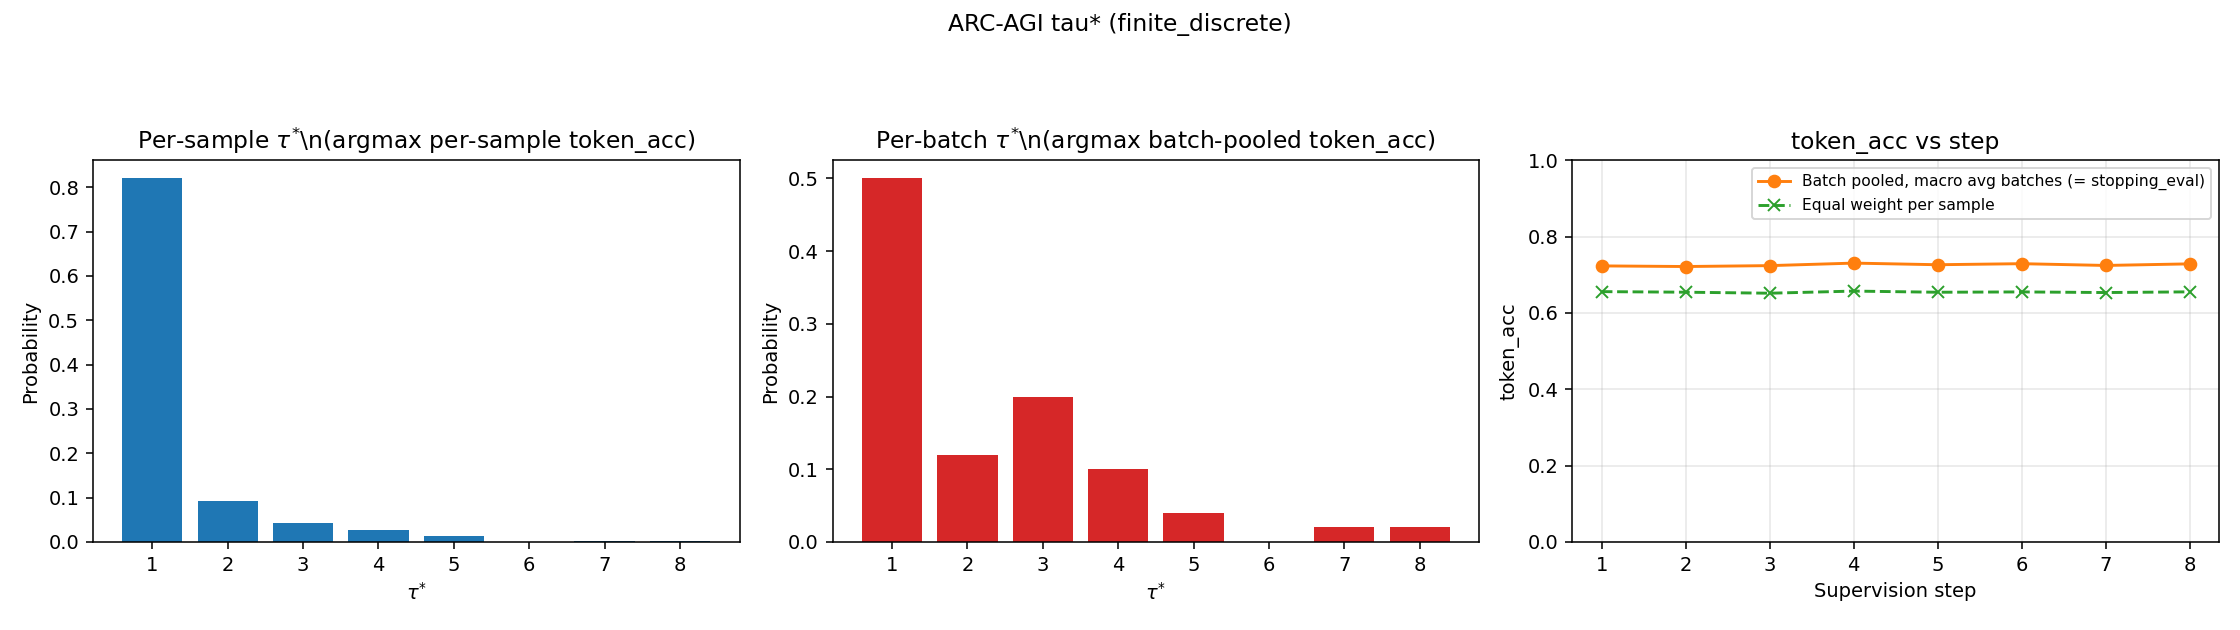
\includegraphics[width=0.88\linewidth]{arc_tau_star_hist_val.png}
\caption{Эмпирическое распределение оракульного \(\tau^\star\) на валидации (ARC-AGI, ветка \texttt{finite\_discrete}).}
\label{fig:arc_tau_hist}
\end{figure}

Численные счётчики и доли по шагам (источник: \texttt{tables/tau\_star\_hist\_finite\_discrete\_val.csv}, согласован с \texttt{tau\_star\_hist\_val.json}) приведены в табл.~\ref{tab:tau_hist_csv}.

\begin{table}[H]
\centering
\caption{Эмпирическое распределение \(\tau^\star\) по шагам (валидация, \texttt{finite\_discrete})}
\label{tab:tau_hist_csv}
\small
\begin{tabular}{r r S[table-format=1.4]}
\toprule
Шаг & Число задач & {Доля} \\
\midrule
\TauHistRows
\bottomrule
\end{tabular}
\end{table}

\subsection{Сводка по семействам распределений (базовое обучение)}

Табл.~\ref{tab:arc_base} агрегирует лучшую по сетке строку для каждого обученного семейства (метрика отбора: \texttt{token\_acc\_best\_of\_policies}). Полный перебор порогов и стратегий хранится в \texttt{stopping\_eval.json} каждого прогона; табличные значения вынесены в \texttt{tables/arc\_stopping\_base.csv}.

\begin{table}[H]
\centering
\caption{ARC-AGI, валидация: лучшая комбинация правила остановки после базового обучения}
\label{tab:arc_base}
\small
\begin{tabular}{l l S[table-format=1.1] S[table-format=1.2] S[table-format=1.5] S[table-format=1.3] S[table-format=1.3]}
\toprule
Семейство & Стратегия & {Порог} & {\(\overline{\tau}\)} & {Регрет} & {\(\mathrm{tok}_{\mathrm{best}}\)} & {\(\mathrm{NLL}_\tau\)} \\
\midrule
\ArcBaseRows
\bottomrule
\end{tabular}
\end{table}

Здесь \(\overline{\tau}=\) \texttt{best\_mean\_steps} --- среднее число внутренних шагов при выбранном правиле; средний регрет --- \texttt{best\_mean\_regret} из сводки; \(\mathrm{tok}_{\mathrm{best}}=\) \texttt{best\_token\_acc\_best\_of\_policies}; \(\mathrm{NLL}_\tau=\) \texttt{best\_nll}. Доля полностью точных решеток на уровне токенов близка к нулю, что ожидаемо для сложной задачи при пошаговой разметке.

\subsection{Влияние дообучения только оракула}

Табл.~\ref{tab:arc_ft} сопоставляет ту же метрику \(\mathrm{tok}_{\mathrm{best}}\) и среднее число шагов до и после \texttt{oracle\_finetune}. Пороги и стратегии переоптимизируются заново на валидации после дообучения. Данные: \texttt{tables/arc\_stopping\_finetune\_compare.csv}.

\begin{table}[H]
\centering
\caption{Сравнение базового чекпойнта и \texttt{oracle\_finetune} (ARC-AGI)}
\label{tab:arc_ft}
\small
\begin{tabular}{l c c S S S S}
\toprule
 & \multicolumn{2}{c}{Стратегия / порог} & \multicolumn{2}{c}{\(\mathrm{tok}_{\mathrm{best}}\)} & \multicolumn{2}{c}{\(\overline{\tau}\)} \\
\cmidrule(lr){2-3}\cmidrule(lr){4-5}\cmidrule(lr){6-7}
Семейство & база & FT & {база} & {FT} & {база} & {FT} \\
\midrule
\ArcFtRows
\bottomrule
\end{tabular}
\end{table}

Для \texttt{smoothed\_loss} дообучение не меняет оптимальную строку сводки. Для \texttt{finite\_discrete}, \texttt{mixture\_geometric} и \texttt{power} оптимальное правило смещается в сторону более агрессивной ранней остановки (\texttt{hazard} или меньший порог \texttt{cumulative\_probability}), при этом \(\mathrm{tok}_{\mathrm{best}}\) меняется незначительно. Для \texttt{negative\_binomial} наблюдается небольшое снижение \(\mathrm{tok}_{\mathrm{best}}\) после дообучения; интерпретация этого факта обсуждается в разд.~\ref{sec:discussion}.

\subsection{Кривая качество--стоимость и калибровка}

Полные кривые «качество--среднее число шагов'' строятся по всем строкам \texttt{stopping\_eval.json} и здесь не приводятся. На рис.~\ref{fig:quality_cost} оставлен лишь шаблон осей: фактические точки получаются при экспорте JSON в скрипт визуализации.

\begin{figure}[H]
\centering
\fbox{\begin{minipage}{0.82\textwidth}
\centering
\vspace{8mm}
\small ось X: среднее число внутренних шагов; ось Y: токеновая точность / потеря; семейства распределений дают разные траектории при изменении порога.
\vspace{8mm}
\end{minipage}}
\caption{Шаблон кривой качество--стоимость (заполнить по \texttt{stopping\_eval.json})}
\label{fig:quality_cost}
\end{figure}

Reliability-диаграммы для событий \(\{\tau^\star\le k\}\) могут быть построены по полям \texttt{brier}, \texttt{ece} из лучших строк сетки; на рис.~\ref{fig:calibration} --- заготовка.

\begin{figure}[H]
\centering
\fbox{\begin{minipage}{0.82\textwidth}
\centering
\vspace{8mm}
\small ось X: предсказанная вероятность; ось Y: эмпирическая частота; диагональ --- идеальная калибровка \cite{guo2017calibration}.
\vspace{8mm}
\end{minipage}}
\caption{Шаблон калибровочной диаграммы для \(\tau^\star\le k\)}
\label{fig:calibration}
\end{figure}

\subsection{Итоговая таблица для языкового трека (плейсхолдер)}

Табл.~\ref{tab:main_results_template} остается для будущего заполнения при подключении языковых прогонов к тому же коду оценки остановки.

\begin{table}[H]
\centering
\caption{Иллюстративный шаблон итогового сравнения на языковой задаче (не измерено в данной работе)}
\label{tab:main_results_template}
\begin{tabularx}{\textwidth}{lYYYYY}
\toprule
Метод & Потеря речи & Доля совпадений & \(\mathrm{NLL}_{\tau}\) & Среднее число шагов & Экономия \\
\midrule
Фиксированная глубина & \placeholder & \placeholder & не применяется & \placeholder & \placeholder \\
Полный запуск рекурсии & \placeholder & \placeholder & не применяется & \placeholder & \placeholder \\
Эвристика по энтропии & \placeholder & \placeholder & не применяется & \placeholder & \placeholder \\
Конечное распределение & \placeholder & \placeholder & \placeholder & \placeholder & \placeholder \\
Сглаженная разметка & \placeholder & \placeholder & \placeholder & \placeholder & \placeholder \\
Смесь геометрических & \placeholder & \placeholder & \placeholder & \placeholder & \placeholder \\
Отрицательное биномиальное & \placeholder & \placeholder & \placeholder & \placeholder & \placeholder \\
\bottomrule
\end{tabularx}
\end{table}

\section{Обсуждение}\label{sec:discussion}

\subsection{Интерпретация свода ARC-AGI}

Лучшие по сетке строки для базового обучения (табл.~\ref{tab:arc_base}) показывают, что наибольшая токеновая точность при выборе между политиками \texttt{last} и \texttt{argmax\_interval} достигается у \texttt{mixture\_geometric} при умеренном среднем числе шагов \(\overline{\tau}\approx 4{,}25\). Семейство \texttt{smoothed\_loss} достигает сравнимой точности при \(\overline{\tau}=K\), то есть фактически без экономии глубины в выбранной оптимальной строке сводки. Семейство \texttt{power} дает конкурентоспособную точность, но с большим регретом, что согласуется с менее жесткой параметризацией хвоста: ошибка распределения времени дороже в смысле~\eqref{eq:oracle_stopping_time}.

\subsection{Дообучение только оракула и сдвиг распределений}

Дообучение только головы оракула при замороженной рекурсивной части меняет не столько предельную токеновую точность при полном прогоне, сколько совместную конфигурацию «распределение \(\rightarrow\) правило остановки''. В табл.~\ref{tab:arc_ft} видно, что для ряда семейств оптимальная стратегия после FT смещается к более ранней остановке при почти неизменной \(\mathrm{tok}_{\mathrm{best}}\). Это можно интерпретировать как \emph{перекалибровку} предсказанных масс \(\widehat p_{t,k}\) по отношению к эмпирическому распределению остаточных ошибок на валидации: правило \texttt{hazard} становится конкурентоспособным, когда отношение \(\widehat p_{t,k}(k)/\sum_{j\ge k}\widehat p_{t,k}(j)\) лучше согласовано с фактическими условными частотами.

Сдвиг распределения \(\tau^\star\) между обучением и валидацией (дрифт) в строгом смысле требует сравнения двух эмпирических мер \(\widehat\nu_{\mathrm{train}}\) и \(\widehat\nu_{\mathrm{val}}\) на \(\{0,\ldots,K\}\), построенных по независимым выборкам задач. В репозитории прямой JSON с параллельной гистограммой train не зафиксирован; качественно дрифт проявляется в различии кривых \texttt{token\_acc} по шагам в \texttt{metrics.jsonl} и в изменении оптимальной строки сводки после FT. Наблюдаемое для \texttt{negative\_binomial} ухудшение \(\mathrm{tok}_{\mathrm{best}}\) после дообучения согласуется с гипотезой локального переобучения головы на train-разметке \(\tau^\star\), не совпадающей с val-режимом сложности; это \emph{гипотеза}, а не следствие теоремы, и проверяется дополнительными регуляризаторами или ранней остановкой FT.

\subsection{Связь с постановкой математической статистики}

С позиций теории решений \cite{ferguson1967} оракул~\eqref{eq:oracle_stopping_time} задает нижнюю границу риска при полной информации, а практическое правило~\eqref{eq:real_stopping_rule} --- это \(\Hh_{t,k}\)-измеримая аппроксимация, чей риск раскладывается на ошибку прогноза \(\tau^\star\) и ошибку остановки по глубине. Разделение оценки полного закона и решающей функции позволяет отдельно измерять калибровку \cite{guo2017calibration} и чувствительность к сдвигу распределения между сплитами.

\section{Заключение}

В работе сформулирована вероятностная постановка задачи выбора времени остановки при рекурсивном прогнозировании речи. Речь рассматривается как случайная последовательность на конечном словаре, а рекурсивная модель строит несколько последовательных распределений следующей языковой единицы. По полной последовательности потерь определяется оракульное время остановки, минимизирующее сумму ошибки и стоимости вычислений.

Основная статистическая задача состоит в оценке условного распределения этого оракульного времени по информации, доступной на текущем внутреннем шаге. Правило остановки отделено от модели распределения. Это позволяет учитывать не только вероятность остановки сейчас, но и вероятность того, что оптимальный момент уже был в прошлом или еще находится впереди.

Рассмотрены шесть семейств распределений на \(\{0,\ldots,K\}\): конечное дискретное, сглаженная целевая разметка по потерям, смесь геометрических, дискретизированная смесь экспоненциальных, степенной спад на отрезке и отрицательное биномиальное распределение. Для принятия решения используются пять правил: накопленная вероятность, малая вероятность будущего улучшения, условная интенсивность по предсказанной мере, квантиль и бюджетное правило.

На данных ARC-AGI приведена сводка валидационных экспериментов по сетке стратегий остановки, эмпирическое распределение оракульного \(\tau^\star\) и сравнение базового обучения с дообучением только головы оракула. Для языкового трека зафиксирована иллюстративная постановка на публичных корпусах с плейсхолдерными численными значениями.

Направления дальнейшей работы: (i) полный языковой свип с тем же протоколом оценки; (ii) формальные оценки дрифта \(\widehat\nu_{\mathrm{train}}\) vs \(\widehat\nu_{\mathrm{val}}\) для \(\tau^\star\); (iii) построение калибровочных кривых по полному массиву \texttt{stopping\_eval.json}.


\clearpage
\printbibliography[title={Список литературы}]

\appendix
\section{Шаблон журнала эксперимента}

Для воспроизводимости каждый запуск должен сопровождаться записью параметров. Минимальная форма приведена в табл.~\ref{tab:run_log}.

\begin{table}[H]
\centering
\caption{Шаблон журнала одного запуска}
\label{tab:run_log}
\begin{tabularx}{\textwidth}{lY}
\toprule
Поле & Значение \\
\midrule
Идентификатор запуска & \todo{строка} \\
Дата запуска & \todo{дата} \\
Корпус & \todo{название} \\
Словарь & \todo{описание} \\
Основа модели & \todo{название малой модели} \\
Максимальное число шагов & \todo{число} \\
Семейство распределения времени & \todo{название} \\
Правило остановки & \todo{название} \\
Порог правила & \todo{число} \\
Коэффициент стоимости & \todo{число} \\
Начальное зерно & \todo{число} \\
Примечания & \todo{кратко} \\
\bottomrule
\end{tabularx}
\end{table}

\section{Минимальный список проверок перед защитой}

Перед включением численных результатов в основной текст нужно проверить четыре вещи. Во-первых, все методы должны использовать один и тот же словарь и одно и то же разбиение данных. Во-вторых, пороги правил остановки должны подбираться только на проверочной выборке. В-третьих, сравнение методов должно проводиться не только при одном пороге, но и при одинаковом среднем бюджете. В-четвертых, для всех таблиц должны быть указаны средние значения по нескольким запускам и разброс результатов.

\end{document}


\end{document}
